\documentclass[11pt]{beamer}
\title{Using Dynamic Analysis to Generate Disjunctive Invariants}
\usepackage{verbatim}
\usepackage{amsmath}
\usepackage{amsthm}
\usepackage{listings}
\usepackage{graphics}
\usepackage{color}
\usepackage{stmaryrd}

\newtheorem{proposition}{Proposition}
\author{ThanhVu Nguyen et al.}
\date{\today}


\begin{document}
\maketitle
\begin{frame}\frametitle{Introduction}
\begin{itemize}
\item Invariants: defect detection, program verification and program repair.

\item Find the invariants: static or dynamic, and their pros and cons.

\item Conjunctive, polynomial and convex invariants $\Rightarrow$ Disjunctive program properties

\end{itemize}

\end{frame}
\begin{frame}\frametitle{Disjunctive Program}
\begin{example}
\[\texttt{if }(p)\{a = 1;\}\texttt{ else }\{a=2;\}\]
\end{example}
Neither $a = 1$ nor $a = 2$ is an invariant, but $(p \wedge a = 1)\vee (\neg p \wedge a = 2)$ is an invariant.
\end{frame}
\begin{frame}\frametitle{Overview}
\begin{itemize}
\item Existing invariant inference algorithm.


\item Max-Plus invariants and a way to infer them.


\item Using $k$-induction to verifying candidate invariants.


\item Experiment results.

\end{itemize}
\end{frame}

\begin{frame}\frametitle{Motivating Example}
\begin{example}[1]
\begin{center}
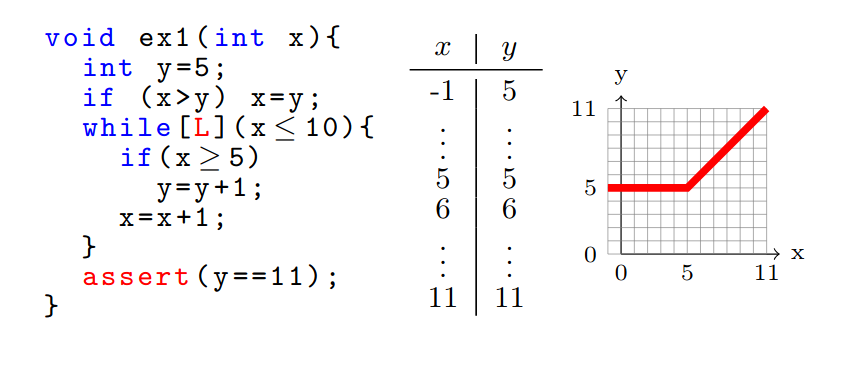
\includegraphics[scale=0.36]{1.png}
A program with branch and a executing trace starting from $x = -1$.
Invariant at location \texttt{L} is 
\[(x < 5 \wedge y = 5) \vee (5 \le x \le 11 \wedge x = y)\]
\end{center}
\end{example}

\end{frame}

\begin{frame}\frametitle{Conjunctive Invariant}
From the given trace, existing tools loke Daikon and DIG can generate conjunctive invariant below:
\[11\ge x\]\[11 \ge y \ge 5\]\[y \ge x\]

which is over-approximating and cannot express the disjunctive behavior.
\end{frame}
\begin{frame}\frametitle{Algorithm Overview}
Max-plus inequality: e.g. $\max(x, y+1) \ge 1$

By constructing a max-plus polyhedra over the trace points, we obtain relations simplified to 
\begin{center}
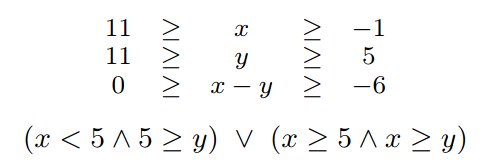
\includegraphics[scale=0.4]{2.png}
\end{center}
Then use $k$\textbf{-induction} to remove the spurious relations $x - y \ge -6, x \ge -1$. Further, the prover proves that $11 \ge x$ is redundant.
\[11 \ge y  \ge 5\]
\[0 \ge x - y\]
\[(x < 5 \wedge 5 \ge y)\vee(x \ge 5 \wedge x \ge y)\]
\end{frame}

\begin{frame}\frametitle{Invariant Inference Algorithm}
DIG: A Dynamic Invariant Generator for Polynomial and Array Invariants

General polyhedra inequality:
\[c_1t_1+\ldots + c_nt_n \ge 0\]

Octagonal Inequalities:
\[c_1t_1 + c_2t_2 \ge k\]



\begin{center}
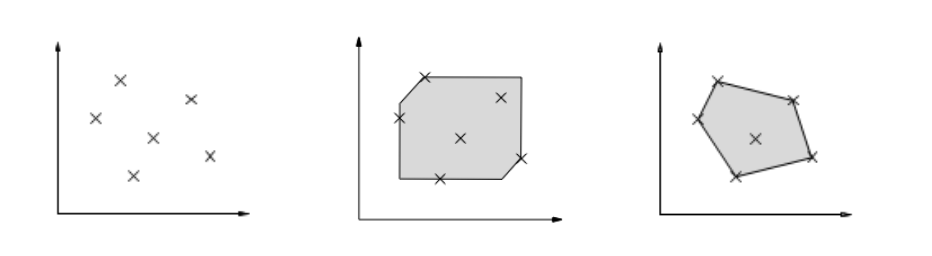
\includegraphics[scale=0.3]{10.png}
\end{center}
\end{frame}

\begin{frame}\frametitle{Max-Plus Invariant}
To model disjunctive invariant, we use formulas representing max-plus polyhedra. i.e. a non-convex hull which is convex in the sense of max-plus algebra. Formally, max-plus relation can be expressed as:
\[\max(c_0, c_1 + v_1, \ldots, c_n + v_n) \ge \max(d_0, d_1 + v_1, \ldots, d_n + v_n)\]

$c_i, d_i\in \mathbb{R} \cup \{-\infty\}$

It is obvious that $\max(x, y) > n$ is equivalent to $(x \ge y \wedge x > n )\vee (y > x \wedge y > n)$. Hence,...
\end{frame}

\begin{frame}\frametitle{Geometric Shape of Max-Plus Invariant}
\begin{center}
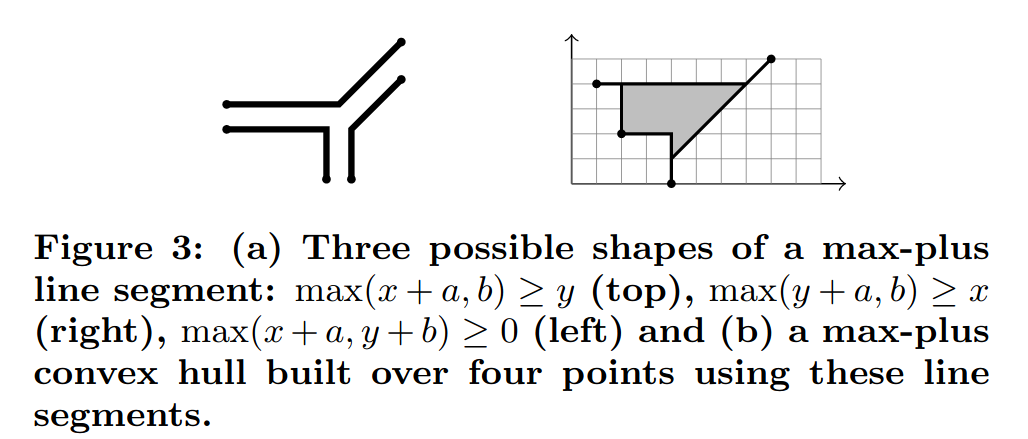
\includegraphics[scale=0.27]{3.png}
\end{center}
Convex on max-plus algebra: for any two points of the max-plus polyhedra, there is a max-plus line segment connecting these two points.
\end{frame}

\begin{frame}\frametitle{Dynamically Infer Max-Plus Invariants }
Input: set of variables $V$, set of traces $X$, max degree $d$

Output: A set $S$ of polynomial inequalities.

$T \leftarrow \texttt{genTerms}(V,d)$

$P \leftarrow \texttt{genPoints}(T,X)$

$H \leftarrow \texttt{createMaxPlusPolyhedron}(P)$

$S\leftarrow \texttt{extractFacets}(H)$

return $S$.
\end{frame}

\begin{frame}\frametitle{Inferring Example}
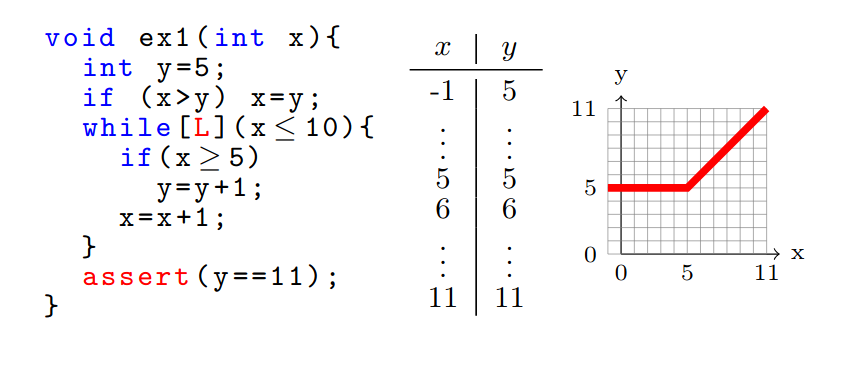
\includegraphics[scale=0.24]{1.png}
\begin{center}
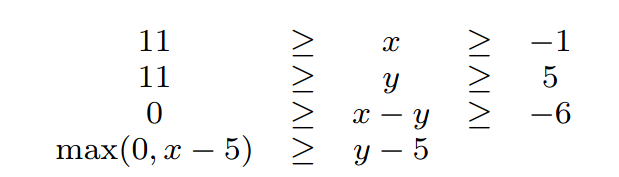
\includegraphics[scale=0.34]{4.png}
\end{center}
Conjunctions of formulas above is equivalent to 
\[(x < 5 \wedge 5 = y) \vee (5 \le x \le 11 \wedge x = y)\]
\end{frame}


\begin{frame}\frametitle{Weak Max-Plus Invariants}
Traditional min max invariant complexity: $O(n^k)$\footnote{Inferring Min and Max Invariants Using Max-plus Polyhedra}.

We define a weak max relation to be of the form: 

\[\max(c_0, c_1 + v_1, \ldots, c_k + v_k) \ge v_j + d\]
\[v_j + d \ge \max(c_0,c_1 + v_1, \ldots, c_k + v_k)\]

where $c_i \in \{0, -\infty\}$

Difference of weak version: 
Only  performs in the form $\max(x, b) \ge y$ and $\max(y, b)\ge x$


\end{frame}

\begin{frame}\frametitle{Example of Finding Weak Max-Plus Invariant}
Points: $\{(x_1, y_1), \ldots, (x_n, y_n)\}$ in 2D. 

For the form $\max(c_0, x + c_1, y + c_2) \ge x + d$, there are 8 versions depending on the value of $c_i$. Same for the other direction and different variable. 

Then compute parameter $d$ by using the points. e.g.
\[\max(y,0)\ge x + d\]
then, $d = \min(\max(y_i, 0) - x_i)$

Number of inequalities: $O(k2^{k+2})$

Time complexity: $O(n2^k)$




\end{frame}

\begin{frame}\frametitle{Min-Plus Invariant}
Min relation is of the form
\[\min(c_0, c_1 + v_1, \ldots, c_n + v_n) \ge \min(d_0, d_1 + v_1, \ldots, d_n + v_n)\]
Shapes:
\begin{center}
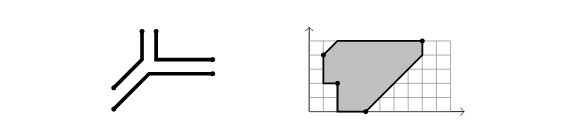
\includegraphics[scale=0.4]{5.png}

\end{center}
Min-plus:
\[\min(c_0, c_1 + v_1, \ldots, c_k + v_k) \ge v_j + d\]
\[v_j + d \ge \min(c_0,c_1 + v_1, \ldots, c_k + v_k)\]

where $c_i \in \{0, +\infty\}$

\end{frame}

\begin{frame}\frametitle{Combine Max-Plus and Min-Plus}
\begin{center}
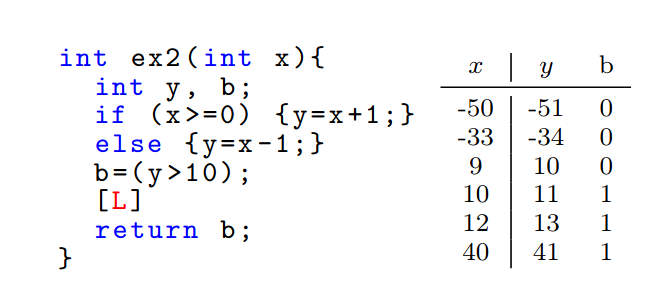
\includegraphics[scale=0.35]{11.png}
\end{center}
The invariant of this program at location $L$ is 
\[y\le 10 \Leftrightarrow b = 0\]
can be described equivalently by 
\[\max(y - 10, 0) \ge b \text{ and } b + 10 \ge\min(y, 11)\]
\end{frame}

\begin{frame}\frametitle{Verifying Candidate Invariant}
In the algorithm we use $k$-induction to verify the invriant and remove spurious invariant.

\textbf{k-Induction:} $k$ base cases are specified, and $k$ previus instance are availble to prove the inductive step.

$M = (I,T)$
\begin{center}
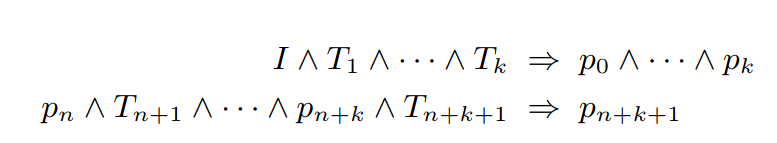
\includegraphics[scale=0.35]{7.png}
\end{center}
Sound, not complete.



\end{frame}

\begin{frame}\frametitle{k-Induction Example}
\begin{example}[2]
$M = (I,T)$

$I: x_0 = 0\wedge y_0 = 1\wedge z_0 = 2$.

$T_n: x_n = y_{n-1} \wedge y_n = z_{n-1} \wedge z_n = x_{n - 1}$
\end{example}

Standard induction: $I\Rightarrow p_0$, $p_i \wedge T_{i+1} \not\Rightarrow p_{i+1}$.

3-Inductive: $I \wedge T_1 \wedge T_2\wedge T_3 \Rightarrow p_0 \wedge p_1\wedge p_2\wedge p_3$.

$p_i\wedge T_{i+1} \wedge p_{i+1}\wedge T_{i+2} \wedge p_{i+2}\wedge T_{i+3} \Rightarrow p_{i+3}$
\end{frame}

\begin{frame}\frametitle{Code: k-Induction}
\begin{center}
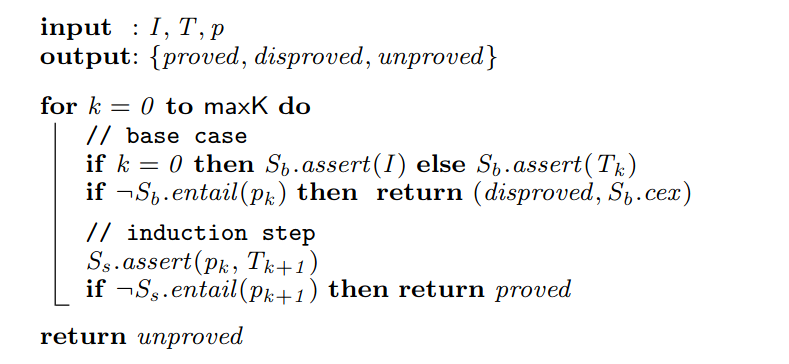
\includegraphics[scale=0.4]{8.png}
\end{center}
\end{frame}

\begin{frame}\frametitle{Code: KIP}
\begin{center}
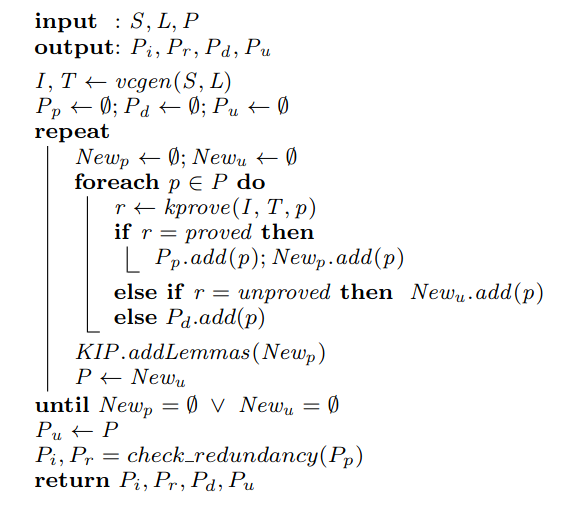
\includegraphics[scale=0.4]{9.png}
\end{center}
\end{frame}

\begin{frame}\frametitle{Experiment Result}
\begin{center}
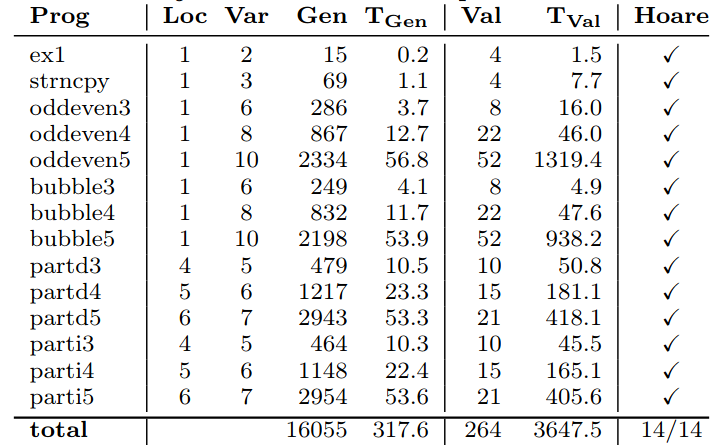
\includegraphics[scale=0.4]{12.png}
\end{center}
\end{frame}
\end{document}